\documentclass[11pt]{article}

\usepackage[spanish,activeacute]{babel}
\usepackage{titlesec}
\usepackage{graphicx}
\usepackage{float}
\usepackage[bottom]{footmisc}
\usepackage[hidelinks]{hyperref}
\usepackage{subcaption}
\usepackage[most]{tcolorbox}
\usepackage{xcolor}


\setlength{\parindent}{1.0em}
\setlength{\parskip}{1.0em}
\setlength{\emergencystretch}{5.0em}
\setlength{\belowcaptionskip}{-10pt}
\counterwithin{figure}{section}
\titlespacing*{\section}{0em}{3.5em}{1.5em}
\setcounter{tocdepth}{2}
\hypersetup{
	linktoc=all
}


\title{\Huge Servidores}
\author{Eugenia Damonte, Ariel Fideleff y Mart\'in Go\~ni}
\date{}


\definecolor{light-orange}{RGB}{168,87,0}
\definecolor{light-blue}{RGB}{64, 76, 201}
\definecolor{dark-gray}{RGB}{100,100,100}
\definecolor{light-red}{RGB}{201, 60, 60}
\definecolor{fuchsia}{RGB}{168,0,168}


\newtcolorbox{code-box}{colback=white!75!gray,colframe=white!15!gray,fontupper=\linespread{1.15}\selectfont}


\newcommand{\imagecaption}[1]{\vspace{-7pt}\caption*{\char91\ref{fig:#1}\char93}}
\newcommand{\codetext}[2]{\large\texttt{\textcolor{#1}{#2}}}


\begin{document}
	\pagenumbering{gobble}
	\maketitle
	\newpage
	\tableofcontents
	\newpage
	\pagenumbering{arabic}
	
	
	\section{puTTY}
	\subsection{Que es puTTY}
		\texttt{puTTY} es una serie de herramientas de c'odigo abierto que permite la transferencia de archivos mediante la red, as'i como tambi'en el acceso a una consola serial, entre otras cosas. Cuando se habla de puTTY de manera general en realidad se est'a hablando de una serie de programas o componentes, desarrollados y mantenidos por el programador brit'anico Simon Tatham. Estos son:
		
		\begin{itemize}
			\item \texttt{puTTY} - Aplicaci'on para utilizar Telnet\footnote{Telnet o \texttt{Teletype Network} es un protocolo de red que permite acceder a la terminal de otra m'aquina de manera remota. Es adem'as el nombre del programa que usa el cliente.}, Rlogin\footnote{Rlogin o \texttt{Remote Login} es una aplicaci'on TCP/IP que inicia una sesi'on de terminal remota en el host especificado.} y un cliente SSH\footnote{Un cliente SSH es un programa que permite establecer conexiones seguras a servidores SSH.}, tambi'en permite la conexi'on a puertos seriales.
			\item \texttt{PSCP} - Cliente que permite realizar \textit{command-line secure file copy}, es decir copiar archivos de manera segura desde un terminal. Puede adem'as hacer transferencias SFTP.
			\item \texttt{PSFTP} - Cliente que permite utilizar SFTP\footnote{SFTP o \texttt{SSH File Transfer Protocol} es un protocolo seguro de transferencia de archivos, hoy en dia ha reemplazado casi completamente a FTP, su predecesor.} para transferir archivos..
			\item \texttt{puTTYtel} - Un cliente espec'ifico para Telnet.
			\item \texttt{Plink} - Una interfaz de consola que permite acceder a el \textit{back end} de puTTY. Normalmente usado para manejar t'uneles SSH\footnote{Un tunel SSH es un m'etodo para transportar informaci'on en la red de manera segura usando una conexi'on SSH encriptada.}.
			\item \texttt{Pageant} - Un agente de autenticaci'on para puTTY, PSCP y Plink.
			\item \texttt{puTTYgen} - Una aplicaci'on que permite generar llaves de encripci'on \texttt{RSA}, \texttt{DSA}, \texttt{ECDSA} y \texttt{EdDSA}.
		\end{itemize}
		
		En nuestro caso estamos interesados solamente en \texttt{puTTY} y \texttt{puTTYgen}, dado que son los necesarios para acceder de manera segura a una m'aquina remota usando SSH.
		
	
	\subsection{Conexi'on inicial}
		Nuestro objetivo con \texttt{puTTY} era usarlo para poder acceder de manera remota a una m'aquina\footnote{En nuestro caso utilizamos nuestra propia m'aquina virtual con \texttt{Debian 7}.} utilizando el protocolo SSH.
				
		Lo primero que hicimos fue crear un puerto por el cual pudi'esemos acceder a la \texttt{VM}, para hacer esto fuimos a la configuraci'on de la misma en \texttt{VirtualBox} y en el men'u \texttt{Network} abrimos las opciones avanzadas, seleccionando \texttt{port forwarding}. En el clickeamos el bot'on con el signo mas para crear una nueva regla de redirecci'on de puertos. Le pusimos \texttt{SSH} de nombre, dejando el protocolo en \texttt{TCP}. \texttt{Host IP} y \texttt{Guest IP} los dejamos vac'ios para que se asignen autom'aticamente al momento de uso, dado que las direcciones IP no son est'aticas. Finalmente completamos los campos correspondientes con los puertos. Para el del \texttt{Host}, es decir el de Windows, utilizamos el 5999 dado que es un puerto raro, haciendo poco probable que este ocupado. Para el puerto del \texttt{Guest}, es decir la VM, usamos el 22, el puerto est'andar usado por SSH.
		
		\begin{figure}[H]
    			\centering
    			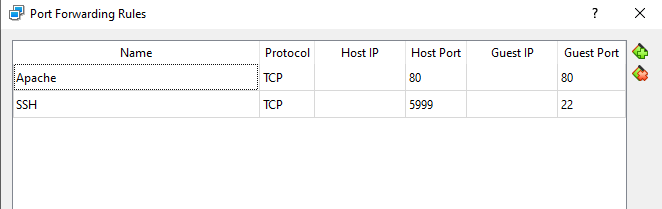
\includegraphics[scale=0.65]{Images/Install/port_forwarding.PNG}
    			\caption{El men'u de \texttt{port forwarding} de nuestra m'aquina virtual.}
    			\label{fig:port_forwarding}
		\end{figure}
		
		Una vez configurados los puertos nos dirigimos a la VM para verificar que los servicios SSH estuviesen funcionando de manera correcta. Para hacer esto usamos dos comandos, el primero \texttt{ps ax | grep ``ssh''} busca procesos con la palabra ``ssh'' en la lista de procesos activos. Al ejecutarlo encontr'o dos, indicando que los servicios estaban funcionando. Luego, para estar seguros utilizamos otro comando \texttt{/etc/init.d/ssh status}, al ejecutarlo nos inform'o, de nuevo, que los servicios SSH estaban funcionando correctamente. 
		
		\begin{figure}[H]
    			\centering
    			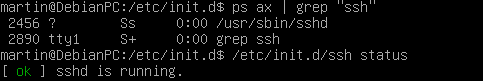
\includegraphics[scale=0.8]{Images/Config/SSH_check.PNG}
    			\caption{Los comandos usados para verificar el funcionamiento de los servicios SSH.}
    			\label{fig:SSH_check}
		\end{figure}
		
		Sabiendo que los servicios SSH estaban funcionando procedimos a realizar el primer intento de conectarnos de manera remota a la VM. Para hacer esto abrimos \texttt{puTTY}, y en el men'u \texttt{Session} pusimos \texttt{localhost} en \texttt{Host Name} y 5999 en \texttt{Port}. El resto de las opciones las dejamos con sus valores predeterminados. Lo que significan estos valores es dentro de la computadora misma(\texttt{localhost}), conectarse al puerto 5999, que es el que especificamos en la configuraci'on de la VM, usando el protoclo SSH.
		
		\begin{figure}[H]
    			\centering
    			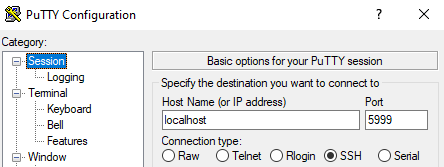
\includegraphics[scale=0.9]{Images/Connection/first_connection_attempt.PNG}
    			\caption{La configuraci'on para la primera conexi'on a la VM.}
    			\label{fig:first_connection_attempt}
		\end{figure}
		
		Habiendo ingresado toda la informaci'on clickeamos el bot'on \texttt{Open} para iniciar la conexi'on con la VM. Al hacerlo apareci'o una consola pidiendo que ingresemos nuestro nombre de usuario, y luego contraseña. Al ingresarlos, se nos concedio acceso, pudiendo usar la consola de \texttt{puTTY} como si fuese la consola de la VM. 
		
		\begin{figure}[H]
    			\centering
    			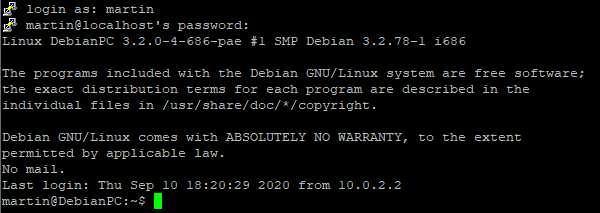
\includegraphics[scale=0.9]{Images/Connection/first_connection_console.PNG}
    			\caption{La primera conexi'on a la VM, hecha usando el protcolo SSH y \texttt{puTTY}.}
    			\label{fig:first_connection_console}
		\end{figure}
		
	\subsection{Conexi'on usando llaves}
		Si bien este m'etodo funciona, ser'ia muy peligroso usarlo para un servidor real. Esto es porque cualquiera podria conectarese a el mismo y obtener acceso al terminal de la m'aquina. Para solucionar este problema usamos una opci'on que tiene el protocolo SSH que permite validar conexiones mediante el uso de un par de llaves de encripci'on, una p'ublica y una privada. La p'ublica se encuentra en la VM, y la privada en la computadora desde la cual se realiza la conexi'on, siendo usada por \texttt{puTTY}.
		
		Lo primero que hay que hacer para usar la autenticaci'on por llaves es generarlas, para esto usamos el prgrama \texttt{puTTYgen}. Una vez abierto bajo la secci'on \texttt{Actions} clickeamos el bot'on \texttt{Generate} sin cambiar niguna de las opciones. Al terminar guardamos la llave privada como \texttt{id\_rca.ppk} y la p'ublica como \texttt{public\_key}.	
		
		\begin{figure}[H]
    			\centering
    			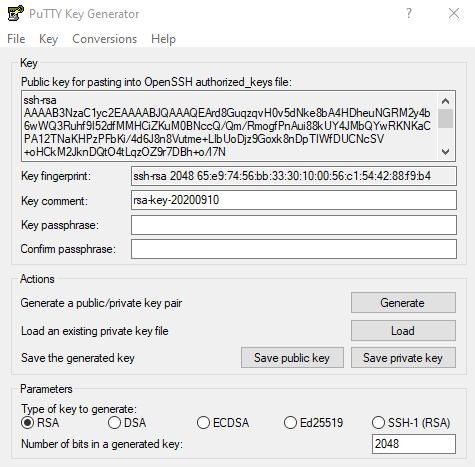
\includegraphics[scale=0.9]{Images/Connection/puTTYgen.PNG}
    			\caption{Configuraci'on de \texttt{puTTYgen} usada para generar las llaves.}
    			\label{fig:puTTYgen}
		\end{figure}
		
		Una vez generadas las llaves ten'iamos que llevar la p'ublica a la VM, as'i como tambi'en cambiar la configuraci'on de SSH para que solo permitiese conexiones con llaves. Para hacer esto volvimos a conectarnos a la VM usando \texttt{puTTY}. Una vez all'i lo primero que hicimos fue ir al directorio escondido \texttt{.ssh} en nuestro directorio propio. All'i creamos un archivo llamado \texttt{autorized\_keys}, en el copiamos la llave p'ublica generada por \texttt{puTTYgen}. 
		
		\begin{figure}[H]
    			\centering
    			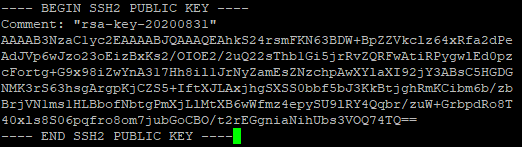
\includegraphics[scale=0.9]{Images/Connection/public_key.PNG}
    			\caption{Llave p'ublica copiada a la VM usando la terminal de \texttt{puTTY}.}
    			\label{fig:public_key}
		\end{figure}
		
		Con la llave p'ublica en la VM era hora de configurar SSH para que solo sea posible la autenticaci'on mediante llaves, no permitiendo usar contrase'nas. Para esto abrimos el archivo \texttt{/etc/ssh/sshd\_config} que es el archivo de configuraci'on de SSH. En el cambiamos cuatro cosas:
		
		\begin{itemize}
			\item Cambiamos \texttt{PubkeyAuthentication} de \texttt{no} a \texttt{yes}.
			\item Descomentamos \texttt{AuthorizedKeyFile    .ssh/authorized\_keys}.
			\item Cambiamos \texttt{PasswordAuthentication} de \texttt{yes} a  \texttt{no}.
			\item Cambiamos \texttt{ChallengeResponseAuthentication} de \texttt{yes} a \texttt{no}.
		\end{itemize}
		
		Para que estos cambios tomen efecto tuvimos que reiniciar los servicios SSH, usando el comando \texttt{sudo /etc/init.d/ssh restart}. Al ejecutarlo nos dijo que los servicios se hab'ian reiniciado correctamente.
		
		\begin{figure}[H]
    			\centering
    			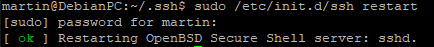
\includegraphics[scale=0.9]{Images/Connection/ssh_restart.PNG}
    			\caption{El comando usado para reiniciar los servicios SSH.}
    			\label{fig:ssh_restart}
		\end{figure}
		
		Para verificar si esto hab'ia funcionado primero era necesario configurar \texttt{puTTY} para utlizar la llave privada. Para hacerlo cerramos la terminal y volvimos a iniciar \texttt{puTTY}. En el men'u \texttt{Session} volvimos a introducir la misma informaci'on que antes. Luego fuimos al men'u \texttt{Data} bajo \texttt{Connection} donde en \texttt{Auto-login username} pusimos el nombre de usuario en la VM. Finalmente fuimos a el submenu \texttt{Auth}, bajo el men'u \texttt{SSH}, que tambi'en esta en \texttt{Connection} y especificamos la ubicaci'on de la llave privada. Para hacer m'as r'apido el conectarse a la VM con \texttt{puTTY} guardamos todas las configuraciones en una sesi'on que llamamos \texttt{Debian 7 2}.
		
		\begin{figure}[H]
			\centering
			\begin{subfigure}[b]{0.45\linewidth}
				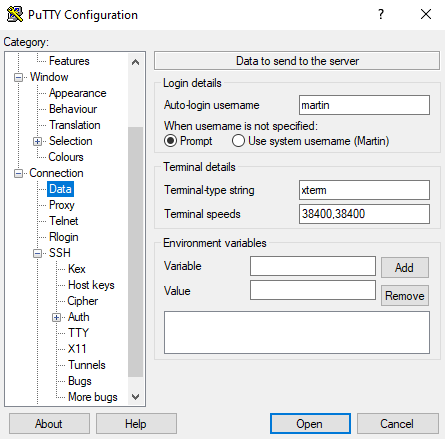
\includegraphics[scale=0.48]{Images/Connection/putty_data.PNG}
			\end{subfigure}
			\begin{subfigure}[b]{0.45\linewidth}
				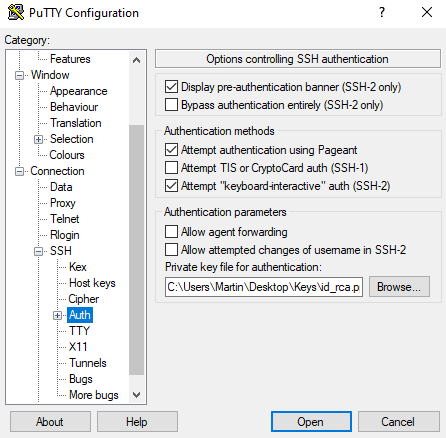
\includegraphics[scale=0.48]{Images/Connection/putty_SSH.PNG}
			\end{subfigure}
			\caption{Configuraci'on de los men'us \texttt{Data} y \texttt{Auth}.}
			\label{fig:putty_configs}
		\end{figure}
		
		Cuando terminamos de ingresar toda la informaci'on apreteamos el bot'on \texttt{Open} para conectarnos con la VM. Mientras se establecia la conexi'on apareci'o una ventana de \texttt{puTTY} diciendo que hab'ia ocurrido un error. Este dec'ia \textit{No supported authentication methods available}, que se traduce como ``No hay metodos de autenticaci'on soportados disponibles''. Esto nos parecio extra'no ya que pareci'a que hab'iamos configurado todo correctamente y no hab'ia mucha informaci'on sobre cual era la causa del error.
		
		\begin{figure}[H]
    			\centering
    			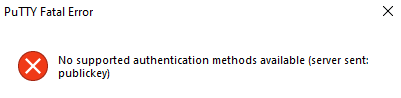
\includegraphics[scale=0.8]{Images/Connection/puTTY_error.PNG}
    			\caption{El error que nos di'o \texttt{puTTY} al intentar conectarnos.}
    			\label{fig:puTTY_error}
		\end{figure}
		
		Luego de investigar un poco descubrimos que la causa del error era como hab'iamos ingresado la llave p'ublica. El formato correcto es \texttt{ssh-rsa (llave)}, estando todo en una misma l'inea.
		
		\begin{figure}[H]
    			\centering
    			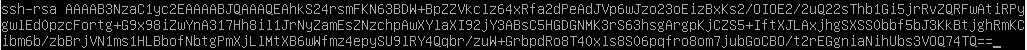
\includegraphics[scale=0.5]{Images/Connection/public_key_final.PNG}
    			\caption{}
    			\label{fig:public_key_final}
		\end{figure}
		
		Luego de solucionar ese problema intentamos conectarnos nuevamente a la VM, cosa que esta vez fue exitosa. Dado que hab'iamos podido conectarnos a nuestra VM desde \texttt{puTTY} utilizando las llaves de manera exitosa decidimos que ya estabamos listos para seguir con el pr'oximo paso, el servidor con Apache.
		
		\begin{figure}[H]
    			\centering
    			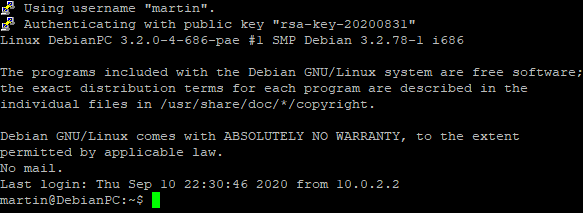
\includegraphics[scale=0.75]{Images/Connection/final_connection.PNG}
    			\caption{Nos conectamos de manera exitosa a la VM.}
    			\label{fig:final_connection}
		\end{figure}
		
		%%%
		
	\section{Servidor web}

		En esta instancia, decidimos instalar y configurar un servidor web: \texttt{Apache HTTP Server}. Un servidor web es un software que permite que un usuario pueda ver el contenido de una p'agina web. A grandes rasgos, lo que sucede al buscar una direcci'on en el navegador es que este busca en qu'e servidor o host se encuentra guardada la p'agina y le ``pide'' el contenido. El servidor web (que est'a instalado en el host) es el encargado de entreg'arselo.

		Lo primero que hicimos para lograr nuestro objetivo fue instalar Apache. Para eso, usamos el comando \texttt{sudo apt-get install apache2}. Verificamos que el servicio anduviera analizando la salida del comando \texttt{ps ax | grep ``apache''}.


		\begin{figure}[H]
    			\centering
   			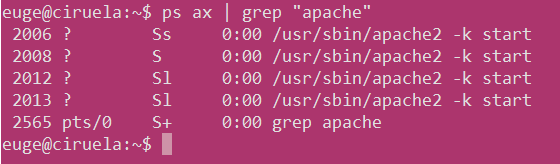
\includegraphics[scale=0.6]{/Images/Apache/fig1}
   			\caption{\texttt{ps ax | grep ``apache''}}
    			\label{fig:1}
		\end{figure}

		Antes de proceder, debimos asegurarnos de no tener un servidor web corriendo en Windows. Si hubi'eramos tenido uno, habr'iamos tenido un problema: os protocolos HTTP usan, por defecto, el puerto TCP 80; si el puerto est'a en uso (si tuvi'eramos otro servidor web), tendr'iamos que redireccionar los puertos y eso llevar'ia m'as trabajo.

		Una forma de asegurarnos de que el puerto 80 est'a libre es correr en el sistema \texttt{telnet localhost 80}. Telnet, como contamos previamente, es un programa que nos permite conectarnos a una computadora remota. La sintaxis de este comando es as'i: \texttt{telnet <servidor>{} <puerto>}. Es decir, al escribir \texttt{telnet localhost 80}, le estamos pidiendo a la computadora que se conecte a su puerto 80. Este paso debe realizarse desde la consola de Windows, no en la m'aquina virtual.

		Algo a resaltar es que es probable que el servicio \texttt{telnet} est'e desactivado en Windows. Para activarlo, simplemente buscamos entre las aplicaciones ``\texttt{Activar o desactivar caracter'isticas de Windows}'' y tildamos el casillero que dice ``\texttt{Telnet Client}''. 

		\begin{figure}[H]
  			\centering
    			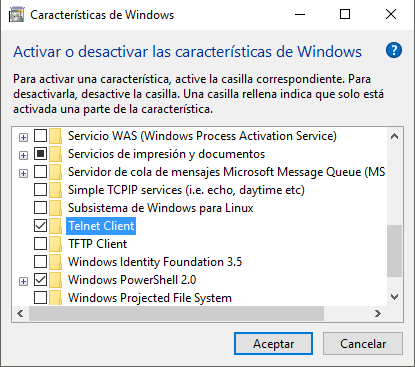
\includegraphics[scale=0.65]{/Images/Apache/fig3}
    			\label{fig:3}
    			\caption{activamos Telnet Client}
		\end{figure}

		Una vez activada esta función, ejecutamos el comando nombrado anteriormente y, si recibimos un error como ``No se puede abrir la conexi'on al host'', quiere decir que no tenemos un servidor web corriendo en este momento en Windows (m'as especificamente, que no estamos usando el puerto 80) y que podremos continuar sin problemas.

		\begin{figure}[H]
    			\centering
    			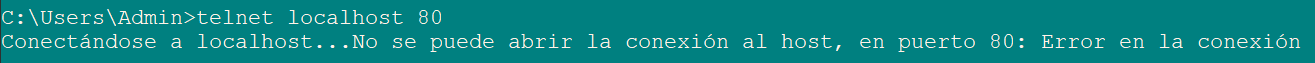
\includegraphics[scale=0.358]{/Images/Apache/fig__}
    			\label{fig:__}
		\end{figure}

		En nuestra m'aquina virtual corremos \texttt{telnet localhost 80} (ahora nos conectamos al puerto 80 de la Virtual Box) y escribimos \texttt{GET / HTTP/1.1}. Presionamos la tecla \texttt{enter} una vez y escribimos \texttt{Host: localhost}. La respuesta deber'ia ser similar a la que se muestra en la imagen \ref{fig:4}.

		\begin{table}[H]
    			\centering
    			\begin{tabular}{|l|}
        			\hline
        			\texttt{GET / HTTP/1.1} \\
        			\texttt{Host: localhost} \\\hline
    			\end{tabular}
    			\label{tab:my_label}
		\end{table}

		\begin{figure}[H]
    			\centering
    			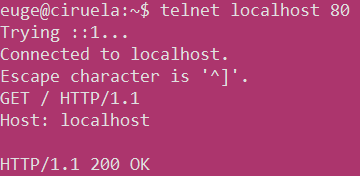
\includegraphics[scale=0.6]{/Images/Apache/fig4_}
    			\caption{pedimos al servidor que nos muestre la p'agina ``/'' y le indicamos que nos comunicamos en HTTP/1.1}
    			\label{fig:4}
		\end{figure}

		Pero ¿qu'e hace el comando ``\texttt{GET / HTTP/1.1}''? \texttt{GET} le pide al servidor el contenido de la p'agina \texttt{/} (una p'agina que es generada por defecto). El 'ultimo argumento que indicamos, \texttt{HTTP/1.1}, es el protocolo y la versi'on del mismo con los que nos comunicamos como cliente. 
Debemos recordar que el pedido que hace el navegador debe ser comprendido por el servidor web. Es decir, deben funcionar en el mismo protocolo: \texttt{HTTP}.
Como primera parte de la respuesta obtuvimos ``\texttt{HTTP/1.1 200 OK}'', que indica que el servidor usa, en este caso, el mismo protocolo que nosotrxs y que nos entiende. La otra parte (no visible en la figura anterior), es el c'odigo \texttt{html} de nuestra p'agina.

		Debemos recordar indicar el \texttt{Host} porque es un requisito de esta versi'on del protocolo y, de lo contrario, obtedr'iamos el error ``\texttt{Bad request}'', el servidor no nos entender'ia. Por otro lado, si escribi'eramos \texttt{GET / HTTP/1.0}, al ser una versi'on m'as vieja, no ser'ia necesario este segundo paso y se entablar'ia la comunicaci'on correctamente, como puede observarse en la figura \ref{fig:5}.

		\begin{figure}[H]
    			\centering
    			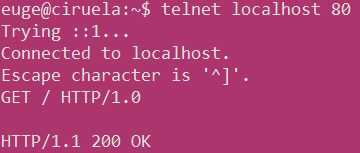
\includegraphics[scale=0.6]{/Images/Apache/fig5_}
    			\caption{pedimos al servidor que nos muestre la p'agina ``/'' y le indicamos que nos comunicamos en HTTP/1.0}
    			\label{fig:5}
		\end{figure}

		S'olo queda configurar los puertos de nuestra m'aquina virtual para que el servidor sea accesible desde otras m'aquinas. Para eso iremos a la aplicaci'on VirtualBox y crearemos una nueva regla de reenv'io de puertos, como hicimos al principio de este trabajo. En el nombre de la regla, indicamos ``Apache''. La configuramos para que tenga protocolo TCP y que los puertos de anfitr'on e invitado sean ambos el 80. Los IPs quedar'an vac'ios para que se acomoden autom'aticamente.

		\begin{figure}[H]
    			\centering
    			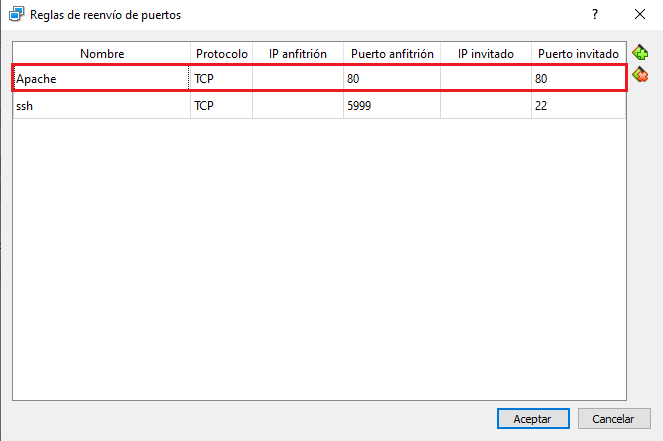
\includegraphics[scale=0.65]{/Images/Apache/fig6}
   			\caption{Caption}
    			\label{fig:6}
		\end{figure}

		Por 'ultimo, entrando a un navegador y usando la direcci'on ``http://localhost'' o simplemente ``localhost'' (tanto en Windows como en la m'aquina virtual), podremos verificar que todo est'e andando bien (en la pantalla dir'a inicialmente  ``It works!'', despu'es podremos editarlo).

		
	\section{Comandos usados}
		A continuaci'on se encuentran todos los comandos utilizados en este trabajo, correspondientes a las im'agenes presentadas.
		
		\begin{figure}[H]
			\centering
			\begin{code-box}
				\codetext{light-blue}{ps} \codetext{light-orange}{ax} \textbar\/ \codetext{light-blue}{grep} \codetext{light-red}{``ssh''}
				
				\codetext{light-blue}{/etc/init.d/ssh} \codetext{light-orange}{status}
			\end{code-box}
			\imagecaption{SSH_check}
		\end{figure}
		
		\begin{figure}[H]
			\centering
			\begin{code-box}
				\codetext{dark-gray}{---- BEGIN SSH2 PUBLIC KEY ----\\
				Comment: ``rsa-key-20200831''\\
				AAAAB3NzaC1yc2EAAAABJQAAAQEAhkS24rsmFKN63BDW+BpZZVkcl
				z64xRfa2dPeAdJVp6wJzo23oEizBxKs2/OIOE2/2uQ22sThb1Gi5j
				rRvZQRFwAtiRPygwlEd0pzcFortg+G9x98iZwYnA317Hh8il1JrNy
				ZamEsZNzchpAwXYlaXI92jY3ABsC5HGDGNMK3rS63hsgArgpKjCZS
				5+IftXJLAxjhgSXSS0bbf5bJ3KkBtjghRmKCibm6b/zbBrjVN1ms1
				HLBbofNbtgPmXjLlMtXB6wWfmz4epySU9lRY4Qqbr/zuW+GrbpdRo
				8T40xls8S06pqfro8om7jubGoCBO/t2rEGgniaNihUbs3VOQ74TQ==\\
				---- END SSH2 PUBLIC KEY ----}
			\end{code-box}
			\imagecaption{public_key}
		\end{figure}
		
		\begin{figure}[H]
			\centering
			\begin{code-box}
				\codetext{fuchsia}{sudo} \codetext{light-blue}{/etc/init.d/ssh} \codetext{light-orange}{restart}
			\end{code-box}
			\imagecaption{ssh_restart}
		\end{figure}
		
		\begin{figure}[H]
			\centering
			\begin{code-box}
				\codetext{dark-gray}{ssh-rsa AAAAB3NzaC1yc2EAAAABJQAAAQEAhkS24rsmFKN63BDW+
				BpZZVkclz64xRfa2dPeAdJVp6wJzo23oEizBxKs2/OIOE2/2uQ22s
				Thb1Gi5jrRvZQRFwAtiRPygwlEd0pzcFortg+G9x98iZwYnA317Hh
				8il1JrNyZamEsZNzchpAwXYlaXI92jY3ABsC5HGDGNMK3rS63hsgA
				rgpKjCZS5+IftXJLAxjhgSXSS0bbf5bJ3KkBtjghRmKCibm6b/zbB
				rjVN1ms1HLBbofNbtgPmXjLlMtXB6wWfmz4epySU9lRY4Qqbr/zuW
				+GrbpdRo8T40xls8S06pqfro8om7jubGoCBO/t2rEGgniaNihUbs3
				VOQ74TQ==}
			\end{code-box}
			\imagecaption{public_key_final}
		\end{figure}
		
		\begin{figure}[H]
			\centering
			\begin{code-box}
				\codetext{fuchsia}{sudo } \codetext{light-blue}{apt-get } \codetext{light-orange}{install } \codetext{dark-gray}{apache2}
			\end{code-box}
			\imagecaption{1}
		\end{figure}
		
		\begin{figure}[H]
			\centering
			\begin{code-box}
				\codetext{light-blue}{ps } \codetext{light-orange}{ax } \codetext{dark-gray}{| } \codetext{light-blue}{grep } \codetext{dark-gray}{``apache''}
			\end{code-box}
			\imagecaption{1}
		\end{figure}

		\begin{figure}[H]
			\centering
			\begin{code-box}
				\codetext{light-blue}{telnet } \codetext{light-orange}{localhost 80}
			\end{code-box}
			\imagecaption{__}
		\end{figure}
		
		\begin{figure}[H]
			\centering
			\begin{code-box}
				\codetext{light-blue}{telnet } \codetext{light-orange}{localhost 80}\newline
				\codetext{light-blue}{GET } \codetext{light-orange}{/ HTTP/1.1}\newline
				\codetext{light-blue}{Host: } \codetext{dark-gray}{localhost}
			\end{code-box}
			\imagecaption{4}
		\end{figure}

























%Remove whitspace when done, for ease of work.
\end{document}
